\documentclass{beamer}
\usetheme{Madrid} % choose from: default	Darmstadt	Malmoe AnnArbor	Dresden	Marburg Antibes	Frankfurt	Montpellier Bergen	Goettingen	PaloAlto Berkeley	Hannover	Pittsburgh Berlin	Ilmenau	Rochester Boadilla	JuanLesPins	Singapore CambridgeUS	Luebeck	Szeged Copenhagen	Madrid	Warsaw
\usecolortheme{spruce} % choose from: wolverine dove spruce beaver albatross {ASP one ;)} 

\usepackage{xcolor, soul}
\definecolor{codegreen}{rgb}{0,0.6,0}
\definecolor{codegray}{rgb}{0.5,0.5,0.5}
\definecolor{codepurple}{rgb}{0.58,0,0.82}
\definecolor{backcolour}{rgb}{0.95,0.95,0.92}

\usepackage{tcolorbox}
\usepackage{listings}
\usepackage{animate}
\usepackage{wrapfig}

\lstdefinestyle{mystyle}{
	backgroundcolor=\color{backcolour},   
	%commentstyle=\color{codegreen},
	keywordstyle=\bfseries,
	numberstyle=\tiny\color{codegray},
	stringstyle=\color{codepurple},
	basicstyle=\footnotesize,
	breakatwhitespace=true,         
	breaklines=true,                 
	captionpos=b,                    
	keepspaces=true,                 
	numbers=left,                    
	numbersep=5pt,                  
	showspaces=false,                
	showstringspaces=false,
	showtabs=false,                  
	tabsize=2
}

\tcbuselibrary{breakable}
\tcbset{%any default parameters
  width=0.7\textwidth,
  halign=justify,
  center,
  breakable,
  colback=white    
}

\usepackage{caption}

\usepackage{tikz}
\usetikzlibrary{arrows.meta, positioning, shapes.geometric, decorations.pathreplacing, fit}


\title{Track Malfunctions in Flatland}
%\subtitle{Subtitle}
\author{Baruch Shteken \and Lena Friedek}
\institute[]{Railway Scheduling, Universität Potsdam \\ \url{https://github.com/wug-on-praat/TRailMix}}

\date{21st Sep 2026}

\begin{document}

\begin{frame}
\titlepage
\end{frame}

%----------------------------------------------------------------

\begin{frame}
	\frametitle{Track Malfunctions}
	\begin{itemize}
		\item real-world issue
		\item negatively affects punctuality
		\item reasons: weather, fires, trespassing, repairs, high-frequent use
	\end{itemize}
	
	% add DB Meme or Fun
	
\end{frame}

%----------------------------------------------------------------

\begin{frame}[fragile]
\frametitle{Malfunctions in Flatland}

\begin{itemize}
	\item \textsf{solve.py} handles train malfunctions.
	
	\item Base encoding for scheduling and forwarding information;
	secondary encoding for rescheduling (Gilkra \cite{Gilkra2025} and Murphy \cite{Murphy2026a}).
	
	\item Information forwarded:
	\begin{itemize}
		\item actions as constraints;
		    \begin{verbatim}
				:- not action(train(0),move_forward,22).
				:- not action(train(1),move_forward,22).
				:- not action(train(1),wait,24).
        	\end{verbatim}
		\item the malfunction atom;
			\begin{verbatim}
				malfunction(1,6,23).
        	\end{verbatim}
		\item \textsf{planned\_action}.
			\begin{verbatim}
				planned_action(train(0),move_forward,0).
				planned_action(train(0),move_forward,1).
        	\end{verbatim}
	\end{itemize}
\end{itemize}

% add picture from output

\end{frame}

%----------------------------------------------------------------

\begin{frame}
	\frametitle{Our Contribution}
	TRailMix \cite{TRailMix2026}
	\begin{itemize}
		\item create malfunction (randomly/deterministically)
		\item forwarding additional information
		\item malfunction logging
		\item visualization in Flatland
	\end{itemize}
	
\end{frame}

%----------------------------------------------------------------
\begin{frame}[fragile]
	\frametitle{Create a Track Malfunction}

	\begin{lstlisting}[style=mystyle, language=Python]
def create_trkmalf(self, timestep, predefined_mals):

	if not predefined_mals:
		malfunction_ind = random.random()

		if malfunction_ind > 0.99:
			malfunction_cell = tuple(random.choice(self.grid))
			malfunction_duration = random.randint(2,20)
			mal_timestep = timestep
			
		else: 
			return([])
	...
	self.track_malfunctions.append((malfunction_cell, malfunction_duration))
	self.track_record.append((malfunction_cell, mal_timestep, malfunction_duration))
	return([(malfunction_cell, malfunction_duration)])
	\end{lstlisting}
	
\end{frame}

%----------------------------------------------------------------

\begin{frame}[fragile]
	\frametitle{Additional Forwarded Information}
	\begin{itemize}
		\item track malfunction 
			\begin{verbatim}
				track_malfunction((17, 19), 21, 13).
			\end{verbatim}
		\item position constraint rules
			\begin{verbatim}
				:- position( _, (17, 19), 14, _).
				:- position( _, (17, 19), 15, _).
			\end{verbatim}
		\item planned position
			\begin{verbatim}
				planned_position(0, (20, 3), 15, s).
				planned_position(1, (28, 25), 15, n).
			\end{verbatim}
		\item current position
			\begin{verbatim}
				current_position(0, (19, 3), 14, s).
				current_position(1, (29, 25), 14, n).
			\end{verbatim}
	\end{itemize}

\end{frame}

%----------------------------------------------------------------

\begin{frame}
    \frametitle{Base and Secondary Encoding Overview}

    \begin{columns}[c]

        % ==================================================
        % LEFT: BASE ENCODING
        % ==================================================
        \begin{column}{0.50\textwidth}
            \centering

            {\textbf{Base Encoding}}

            \vspace{0.2cm}

            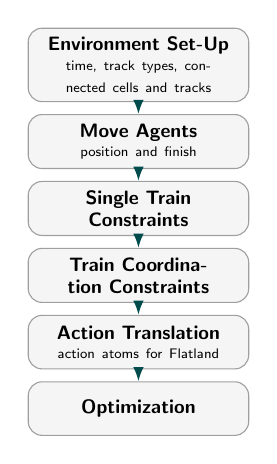
\begin{tikzpicture}[
                box/.style={
                    draw=gray!75,
                    fill=gray!8,
                    rounded corners=5pt,
                    minimum width=2.8cm,
                    minimum height=0.68cm,
                    text width=2.5cm,
                    align=center,
                    font=\sffamily\scriptsize
                },
                container/.style={
                    draw=gray!75,
                    fill=gray!3,
                    rounded corners=7pt,
                    inner sep=6pt
                },
                arrow/.style={
                    -{Latex[length=1.8mm]},
                    draw=teal!60!black,
                    line width=0.7pt
                },
                node distance=0.15cm
            ]

            \node[box] (setup) {
                \textbf{Environment Set-Up}\\[-1pt]
                {\tiny time, track types, connected cells and tracks}
            };

            \node[box, below=of setup] (move) {
                \textbf{Move Agents}\\[-1pt]
                {\tiny position and finish}
            };

            \node[box, below=of move] (train) {
                \textbf{Single Train Constraints}
            };

            \node[box, below=of train] (coordination) {
                \textbf{Train Coordination Constraints}
            };

            \node[box, below=of coordination] (translation) {
                \textbf{Action Translation}\\[-1pt]
                {\tiny action atoms for Flatland}
            };

            \node[box, below=of translation] (optimization) {
                \textbf{Optimization}
            };

            \draw[arrow] (setup) -- (move);
            \draw[arrow] (move) -- (train);
            \draw[arrow] (train) -- (coordination);
            \draw[arrow] (coordination) -- (translation);
            \draw[arrow] (translation) -- (optimization);

            \end{tikzpicture}

        \end{column}


        % ==================================================
        % RIGHT: SECONDARY ENCODING
        % ==================================================
        \begin{column}{0.50\textwidth}
            \centering

            {\textbf{Secondary Encoding}}

            \vspace{0.2cm}

            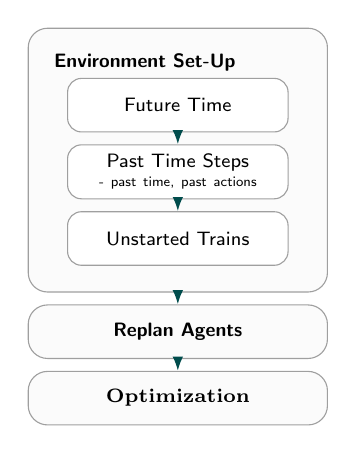
\begin{tikzpicture}[
                box/.style={
                    draw=gray!75,
                    fill=white,
                    rounded corners=5pt,
                    minimum width=2.8cm,
                    minimum height=0.68cm,
                    text width=2.5cm,
                    align=center,
                    font=\sffamily\scriptsize
                },
                container/.style={
                    draw=gray!75,
                    fill=gray!3,
                    rounded corners=7pt,
                    inner sep=6pt
                },
                arrow/.style={
                    -{Latex[length=1.8mm]},
                    draw=teal!60!black,
                    line width=0.7pt
                },
                node distance=0.15cm
            ]

            % ------------------------------------------
            % Environment Set-Up
            % ------------------------------------------
            \node[
                container,
                minimum width=3.8cm,
                minimum height=3.35cm
            ] (setup2) {};

            \node[
                anchor=north west,
                font=\sffamily\scriptsize
            ] at ([xshift=6pt,yshift=-6pt]setup2.north west)
            {\textbf{Environment Set-Up}};

            % Future Time
            \node[box] (future)
                at ([yshift=-28pt]setup2.north)
                {Future Time};

            % Past Time Steps
            \node[
                box,
                below=0.15cm of future
            ] (past)
            {Past Time Steps\\[-1pt]
             {\tiny - past time, past actions}};

            % Unstarted Trains
            \node[
                box,
                below=0.15cm of past
            ] (trains)
            {Unstarted Trains};

            % Arrows
            \draw[arrow] (future) -- (past);
            \draw[arrow] (past) -- (trains);

            % ------------------------------------------
            % Replan Agents
            % ------------------------------------------
            \node[
                container,
                minimum width=3.8cm,
                minimum height=0.68cm,
                below=0.15cm of setup2.south
            ] (replan) {};

            \node[
                font=\sffamily\scriptsize
            ] at (replan.center)
            {\textbf{Replan Agents}};

            \draw[arrow] (setup2) -- (replan);

            % ------------------------------------------
            % Optimization
            % ------------------------------------------
            \node[
                container,
                minimum width=3.8cm,
                minimum height=0.68cm,
                below=0.15cm of replan.south
            ] (optimize)
            {\textbf{\scriptsize Optimization}};

            \draw[arrow] (replan) -- (optimize);

            \end{tikzpicture}

        \end{column}

    \end{columns}

\end{frame}


%----------------------------------------------------------------

\begin{frame}[fragile]
	\frametitle{Rescheduling}
	The basis of our secondary encoding is to determine which 
	trains are affected by the malfunction
	and reschedule only them unless there is a collision
	and then reschedule also the trains affected by the collision
	\begin{small}
	\begin{itemize}
		\item Check if there is a consequence
			\begin{verbatim}
consequence(train(ID), P, T) :- planned_position(ID, P, T, _),
track_malfunction(P, Dur_mal, T_mal), Dur_mal + T_mal >= T.\end{verbatim}
		\item Use as many planned trains as possible
			\begin{verbatim}
{planned(ID)}:- train(ID), not consequence(train(ID), _, _).
#maximize { 1@3, ID : planned(ID)}.\end{verbatim}
		\item Recalculate schedule for unplanned trains
			\begin{verbatim}
calculate(ID) :- consequence(train(ID), _, _).
calculate(ID) :- train(ID), not planned(ID).\end{verbatim}	
	\end{itemize}
	\end{small}

% show the clingo code for this OR add diagram
\end{frame}

%----------------------------------------------------------------

\begin{frame}[fragile]
	\frametitle{Experiment 1 - Heuristic vs. no heuristic}
	\begin{itemize}
		\item Does the Heuristic improve solving?
		\item prefer planned trains:
		\begin{verbatim}
			#heuristic planned(ID): train(ID). [100, true] \end{verbatim}
		\vspace{0.7cm}
		\item \textbf{Results - Yes!}
		\begin{itemize}
			\item small environments: no difference
			\item big/dense environments: heuristic significantly faster (especially in no consequence scenarios - 4~mins)
			\item[->] less re-proving necessary
		\end{itemize}
	\end{itemize}
	
\end{frame}

%----------------------------------------------------------------

\begin{frame}[fragile]
	\frametitle{Experiment 2 - Base vs. Secondary}
	\begin{itemize}
		\item Is Secondary really better than Redo Planning (Waldow \cite{waldow2025})?

		\vspace{1cm}
		\item \textbf{Results - Yes!}
		\begin{itemize}
			\item small environments: little/ no difference
			\item big/dense environments: secondary encoding significantly faster (2~mins in no consequence)
			\item[->] successful use of forwarded information
		\end{itemize}
	\end{itemize}
	
\end{frame}

%----------------------------------------------------------------
\begin{frame}[fragile]
	\frametitle{Prioritization}
	The encodings are different only in their optimization rule prioritization
	\begin{itemize}
		\item First Plan Prioritization
		\begin{verbatim}
			#maximize { 1@3, ID : planned(ID)}.
			#minimize { 1@2, ID, T : action(train(ID), _, T) }.\end{verbatim}
		\item Time Prioritization
		\begin{verbatim}
			#maximize { 1@2, ID : planned(ID)}.
			#minimize { 1@3, ID, T : action(train(ID), _, T) }.\end{verbatim}
	\end{itemize}
	
\end{frame}

%----------------------------------------------------------------

\begin{frame}[fragile]
	\frametitle{Experiment 3 - Base vs. Time Prio}
	\begin{itemize}
		\item Is Secondary with Time Prioritization better than Redo Planning?
		
		\vspace{1cm}
		\item \textbf{Results - Yes??}
		\begin{itemize}
			\item no consequence: base is faster (40~s in large, dense environment) or similar
			\item other consequences: secondary is significantly faster (50\% in a complex scenario)
			\item[->] Time Prio struggles with direct translation of original plan
		\end{itemize}
	\end{itemize}
	
\end{frame}

%----------------------------------------------------------------

\begin{frame}
	\frametitle{Experiment 4 - First Plan vs. Time Prioritization}
	\begin{itemize}
		\item Is Time Prioritization better than First Plan Prioritization?
		
		\vspace{1cm}
		\item \textbf{Results - No!}
		\begin{itemize}
			\item first plan encoding is significantly faster in almost all environments and scenarios
			\item similar performance in small environments
			\item[->] First Plan Prio is faster BUT...
		\end{itemize}
	
	\end{itemize}
	
\end{frame}

%----------------------------------------------------------------

\begin{frame}{Purple Train}
\begin{figure}
	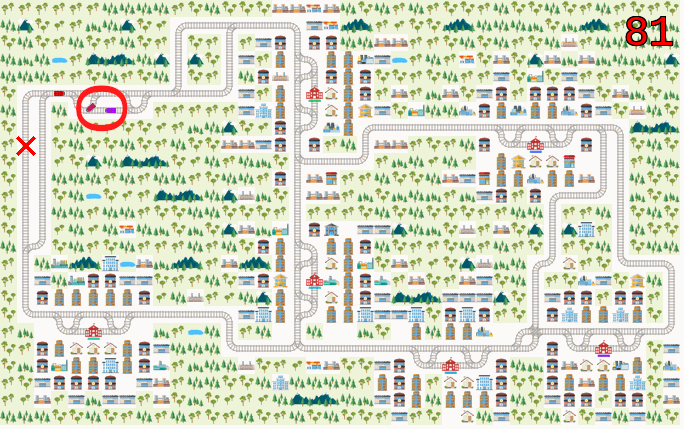
\includegraphics[width=0.8\linewidth]{frame-081_edited.png}
	\caption{Qualitative differences between encodings.}
\end{figure}
\end{frame}


\begin{frame}
	\frametitle{Discussion}
		\begin{figure}[H]
		\centering
		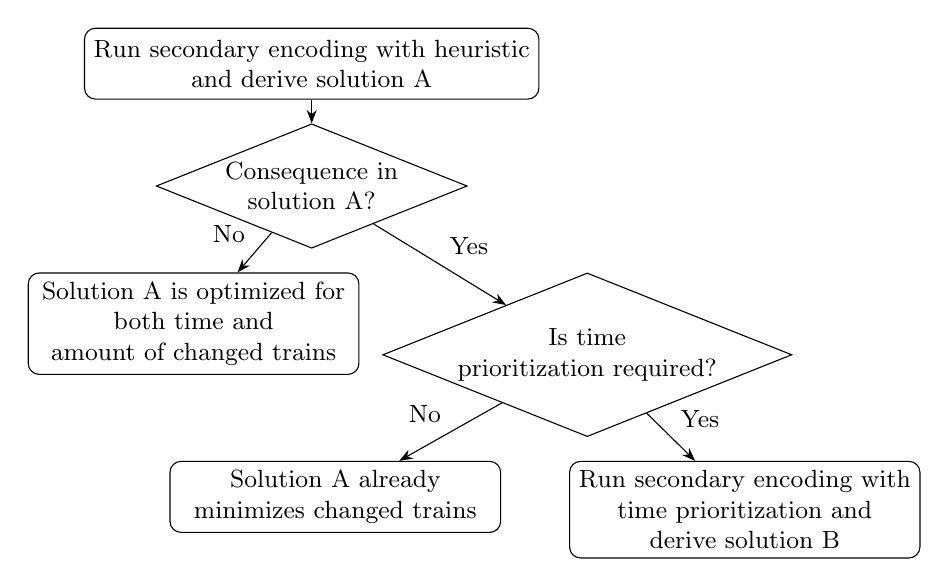
\begin{tikzpicture}[
			node distance=0.3cm,
			every node/.style={font=\small},
			process/.style={
				rectangle,
				rounded corners,
				draw,
				align=center,
				minimum width=4.2cm,
				minimum height=0.9cm
			},
			decision/.style={
				diamond,
				draw,
				align=center,
				aspect=2.5,
				inner sep=1pt
			},
			arrow/.style={
				-{Stealth}
			}
			]
			
			% Start
			\node[process] (start)
			{Run secondary encoding with heuristic\\
				and derive solution A};
			
			% First decision
			\node[decision, below=of start] (consequence)
			{Consequence in\\
				solution A?};
			
			% No consequence branch
			\node[process, below=of consequence, xshift=-1.5cm] (no)
			{Solution A is optimized for\\
				both time and\\
				amount of changed trains};
			
			% Consequence branch
			\node[decision, below=of consequence, xshift=3.5cm] (goal)
			{Is time \\
				prioritization required?};
			
			% Least changed trains
			\node[process, below=of goal, xshift=-3.2cm] (least)
			{Solution A already\\
				minimizes changed trains};
			
			% Most optimized
			\node[process, below=of goal, xshift=2.0cm] (optimized)
			{Run secondary encoding with\\
				time prioritization and\\
				derive solution B};
			
			% Arrows from start
			\draw[arrow] (start) -- (consequence);
			
			% Consequence branches
			\draw[arrow] (consequence)
			-- node[above left] {No} (no);
			
			\draw[arrow] (consequence)
			-- node[above right] {Yes} (goal);
			
			% User goal branches
			\draw[arrow] (goal)
			-- node[above left] {No} (least);
			
			\draw[arrow] (goal)
			-- node[above right] {Yes} (optimized);
			
		\end{tikzpicture}
		\label{fig:rescheduling-encoding-selection}
		\end{figure}
	
\end{frame}

%----------------------------------------------------------------

\begin{frame}
	\frametitle{Future Work}
	\begin{itemize}
		\item Add different random approaches to track malfunctions, e.g frequented tracks might be more prone to a malfunction
		\item Seperate scheduling and rescheduling processes in order to run rescheduling without the scheduling part
		\item Enhance to code to accept the creation of multiple track malfunction per timestep
		\item Visualize the scheduling answer if no rescheduling answer is possible
	\end{itemize}
	
\end{frame}

%----------------------------------------------------------------

\begin{frame}
	\frametitle{References}
	\bibliography{refs.bib}
	\bibliographystyle{splncs04.bst}
\end{frame}

\end{document}